% Exposé II (introduction) and II.A: the image germ; initialisations, pointings and strata.
% Sources: theory/framework.md (Exposé II, II.A), site/sections/03-image.html, theory/propositions.json.
\section{The image germ: expressivity}\label{sec:image}

Expressivity is read off the germ of a method's image at the pretrained point. An initialisation decides whether that
point sits at the apex of a cone, on a smooth sheet of one, or just off the image.

Exposé~\ref{sec:slice} turned a PEFT method into a pointed map $\rho:(Q,q_0)\to(\Theta,\theta_0)$. Its image
$\Im M=\rho(Q)$ is everything it can reach. Fine-tuning travels only a short way from the pretrained weights, so what
matters is the image near $\theta_0$, its \emph{germ} at $\theta_0$ (\bgref{C.8}).

The germ takes few shapes (Figure~\ref{fig:teaser}). It is a linear space when $\rho$ is affine, as for BitFit
\citep{benzaken2021bitfit}, LoRA-FA \citep{zhang2023lora}, LoRA-XS \citep{baazy2024lora}, FourierFT
\citep{gao2024parameter} and (IA)$^3$ \citep{liu2022few}. It is a cone (\bgref{C.10}) when $\rho$ is multihomogeneous
and non-linear and starts where the update vanishes, as LoRA's $BA$ \citep{hu2021lora} does at zero initialisation. It
is a piece of a group orbit for exactly orthogonal methods such as exact-Cayley OFT \citep{qiu2023controlling}. DoRA
\citep{liu2024dora} adds an output gain to LoRA's cone (\thmref{Proposition}{II.8}), and HRA \citep{yuan2024bridging}
meets that cone with a rotation orbit (\thmref{Theorem}{II.7}), each under its stated hypotheses. Adapters and prefixes
change the network itself, and their germs live among functions (Exposé~\ref{sec:merge}).

Four invariants of the germ carry most of the story, and isomorphic methods share them (\thmref{Observation}{I.6}).
\begin{itemize}
  \item The \textbf{first-order image} $S_1(M)=d\rho_{q_0}(T_{q_0}Q)$, the directions a first step can take.
  \item The \textbf{type of the base point}: \emph{regular} when the first-order deficit $d(M)-\dim S_1(M)$ vanishes,
    an \emph{apex} when it is positive (\thmref{Definition}{I.5}).
  \item The \textbf{maximum rank} of an update, bounded by a minimum cut (\thmref{Theorem}{II.10}).
  \item The \textbf{expressive dimension} $d(M)=\dim\Im M$, which falls short of the parameter count $|M|$ by the
    gauge waste $g(M)=|M|-d(M)$.
\end{itemize}

Subsection~\ref{sec:strata} asks where a method starts, Subsection~\ref{sec:erlangen} what a group-type method can never
change (\thmref{Theorem}{II.5}, \thmref{Corollary}{II.6}), and Subsection~\ref{sec:cut} how rank differs from dimension
(\thmref{Proposition}{II.12}). Expressivity here means reach, and finding a reachable point is left to
Exposé~\ref{sec:fibres}.

Which functions a LoRA-adapted network can represent is studied by \citet{zeng2023expressive}. The intrinsic dimension
of \citet{li2018measuring} and \citet{aghajanyan2020intrinsic} depends on the data, while $d(M)$ is a property of the
method alone.

% ======================================================================================================================
\subsection{Initialisations: pointings and strata}\label{sec:strata}

Every LoRA recipe decides where training starts. LoRA \citep{hu2021lora} sets $B_0=0$ and draws $A_0$ at random. PiSSA
\citep{meng2024pissa} takes both factors from the top of the SVD of $W_0$ and subtracts their product from the frozen
weight, LoRA-GA \citep{wang2024lorab} does the same with the first gradient, and CorDA \citep{yang2024corda}, OLoRA
\citep{buyukakyuz2024olora}, MiLoRA \citep{wang2024milora} and EVA \citep{paischer2024parameter} choose otherwise. Each
recipe is a \emph{pointing}, a parameter $q_0$ with the frozen residual that makes $\rho(q_0)=\theta_0$, and two
pointings of one formula can be different objects of $\Meth(\Theta,\theta_0)$. Figure~\ref{fig:apex} draws the typical
cases.

The answers occupy the rest of this subsection. For $r<\min(m,n)$, full-rank LoRA initialisations come in exactly three
kinds up to reparametrisation, classified as sets by $\operatorname{row}A_0$ (when $B_0=0$), by $\operatorname{col}B_0$
(when $A_0=0$) or by the subtracted product $B_0A_0$ (PiSSA-type splits), as \thmref{Theorem}{II.2} shows. Zero-factor
starts sit at the apex of a cone with $mr$ or $nr$ first-order directions, and split starts at a smooth point with all
$r(m+n-r)$. For a $4096\times4096$ matrix at rank $16$ that is $130{,}816$ against $65{,}536$
(\thmref{Proposition}{II.3}). Neither kind reaches everything the other reaches. No exact start of LoRA$_r$ reaches an
update of rank above $2r$ (\thmref{Theorem}{II.1}), and a factor behind a closed gate, such as $A$ when $B_0=0$, does
not move the weights at first order (\thmref{Lemma}{II.4}).

\begin{figure}[tbp]
  \centering
  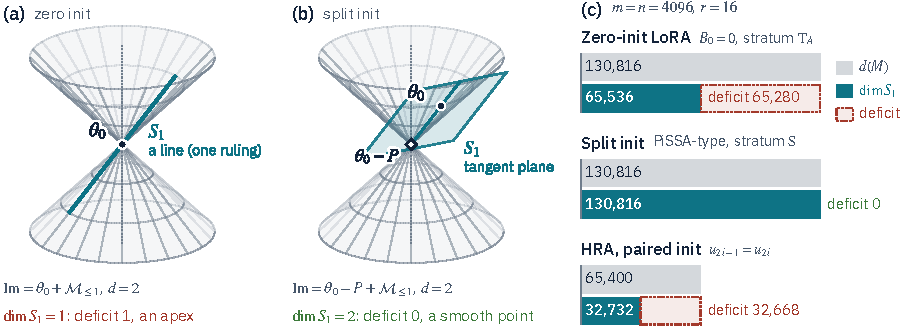
\includegraphics[width=\linewidth]{figures/apex}
  \caption{\textbf{The apex and the smooth point.} Panels (a) and (b) draw the symmetric slice $S=\left(\begin{smallmatrix}x+y&z\\ z&x-y\end{smallmatrix}\right)$ of $2\times2$ matrices, in which rank $\le1$ is the grey double cone $x^2=y^2+z^2$, and the model $\rho(c,\phi)=W_{\rm res}+c\,v_\phi v_\phi\T$, $v_\phi=(\cos\phi,\sin\phi)$, which plays LoRA ($c$ for $B$, $v_\phi$ for $A$); its image is the whole cone, so $d=2$. (a)~Zero initialisation, $c_0=0$ and $W_{\rm res}=\theta_0$: the base point $\theta_0$ is the vertex of the cone, and the first-order image $S_1$ (teal) is a single line, one ruling, so the deficit is $1$ and $\theta_0$ is an apex (\thmref{Definition}{I.5}, \thmref{Theorem}{II.2}(c)). (b)~A split (PiSSA-type) initialisation, $c_0\ne0$ and $W_{\rm res}=\theta_0-P$ with $P=c_0v_{\phi_0}v_{\phi_0}\T$: the vertex moves to $\theta_0-P$ (open diamond), $\theta_0$ lies on a smooth sheet of the cone, and $S_1$ is the tangent plane there, so the deficit is $0$. Both values of $\dim S_1$ are Jacobian ranks of the model. (c)~For $m=n=4096$ and $r=16$, each pair of bars compares the expressive dimension $d(M)$ (grey) with $\dim S_1$ (teal); the dashed red box is the gap between them, the first-order deficit. Zero-init LoRA, stratum $\mathrm T_A$, has $\dim S_1=mr=65{,}536$ against $d=r(m+n-r)=130{,}816$; a split initialisation has $\dim S_1=d$ (\thmref{Theorem}{II.2}(b)); HRA's paired initialisation $u_{2i-1}=u_{2i}$, $k=r/2$, has $\dim S_1=kn-\tfrac{k(k+1)}2=32{,}732$ against $d=rn-\tfrac{r(r+1)}2=65{,}400$, so it too starts at an apex (\thmref{Theorem}{II.7}(b)). The script checks each closed form against a Jacobian rank at $(m,n,r)=(11,9,4)$.}
  \label{fig:apex}
\end{figure}

% ----------------------------------------------------------------------------------------------------------------------
\subsubsection{Translates of one shape}\label{sec:strata-translates}

An additive method adds updates from a fixed shape $C$, for LoRA the cone $\Mr$ of matrices of rank at most $r$
(\bgref{C.12}). Pointing it at $q$ slides the shape so that $\delta(q)$ lands on $\theta_0$, and reachable updates
become differences of two points of $C$ (\bgref{B.14}).

\begin{theorem}{II.1}{pointings of an additive method}
Let $M=(Q,q_0,\theta_0+\delta)$ be additive with shape $C=\delta(Q)$. Write $-v+C$ for a translate, and
$C-C:=\{c-c':c,c'\in C\}$ for the Minkowski difference.

(a) For each $q\in Q$, the re-pointed method $M_q:=(Q,q,\theta_0-\delta(q)+\delta(\cdot))$, with frozen residual
$\theta_0-\delta(q)$, is pointed at $\theta_0$, and $\Im M_q=\theta_0+(-\delta(q)+C)$.

(b) $\bigcup_q\Im M_q=\theta_0+(C-C)$.

(c) For LoRA$_r$ on a single linear box with $s\ne0$, $C-C=\MM_{\le\min(2r,m,n)}$; for several boxes, $C-C$ is the
product of the per-box varieties $\MM_{\le\min(2r,m_i,n_i)}$. Hence \textbf{no exact pointing of LoRA$_r$ (frozen
residual $\theta_0-\delta(q)$), whether zero-init or split (PiSSA, OLoRA, CorDA, LoRA-GA), makes an update
$\theta-\theta_0$ of rank $>2r$ reachable in any adapted matrix.} More robustly, from \emph{any} starting point $q_0$ of
LoRA$_r$, pointed or not, $\rho(q)-\rho(q_0)=\delta(q)-\delta(q_0)$ has rank $\le\min(2r,m,n)$. Quantised-residual
schemes (QLoRA, LoftQ, QPiSSA) are pointed only up to a defect that depends on the order of operations ($e$ for QLoRA;
\thmref{Proposition}{V.2}(b) for the others). Measured from $\theta_0$ rather than from their starting weight, their
updates contain this defect, whose rank is generically at least $\min(m,n)-r$. The bound $2r$ is attained by split
pointings when $2r\le\min(m,n)$.
\end{theorem}

The theorem is elementary, and its rank-$2r$ consequence is known in practice. \citet{meng2024pissa} convert a trained
PiSSA adapter into a rank-$2r$ LoRA through
\begin{equation}\label{eq:pissa-to-lora}
  BA-B_0A_0=\begin{bmatrix}B & B_0\end{bmatrix}\begin{bmatrix}A\\ -A_0\end{bmatrix},
\end{equation}
and HF PEFT ships the conversion. The theorem adds that the conversion loses nothing and that rank $2r$ is needed in
general.

\begin{explains}
An initialisation of an additive method chooses which \emph{translate} of the shape passes through $\theta_0$.
Splitting initialisations (PiSSA-type) buy ``spectral replacement'' updates $Y-P$, which can have rank $2r$. They pay by
losing generic updates of every rank $\ge1$ (\thmref{Theorem}{II.2}(d)). Moving a weight matrix by more than rank $2r$
needs rebasing, as in ReLoRA \citep{lialin2023relora} (\thmref{Theorem}{V.3}), or another shape.
\end{explains}

% ----------------------------------------------------------------------------------------------------------------------
\subsubsection{Three strata}\label{sec:strata-three}

Isomorphisms of methods are pointed diffeomorphisms over $\Theta$ (\thmref{Definition}{I.2}), such as the gauge
$(B,A)\mapsto(Bg^{-1},gA)$ with $g\in\GL_r$ (\bgref{D.21}). They preserve the image and $S_1$
(\thmref{Observation}{I.6}) but may change training (Exposé~\ref{sec:fibres}). Up to isomorphism, a full-rank LoRA
initialisation is determined by one subspace or one matrix.

\begin{theorem}{II.2}{three strata of LoRA initialisations}
Let $\delta(B,A)=BA$ with $1\le r<\min(m,n)$. Consider pointed LoRA objects in three distinguished strata of full-rank
pointings (pointings whose nonzero factors have full rank). Only $\mathrm S$ is open and dense in the space of
pointings; $\mathrm T_A$ and $\mathrm T_B$ are nowhere dense.
\begin{itemize}
  \item $(\mathrm T_A)$: $B_0=0$ and $\rk A_0=r$;
  \item $(\mathrm T_B)$: $A_0=0$ and $\rk B_0=r$;
  \item $(\mathrm S)$: $\rk B_0A_0=r$, with frozen residual $\theta_0-B_0A_0$.
\end{itemize}

(a) \textbf{Classification.} Within a stratum, $M_{q_0}\cong M_{q_0'}$ if and only if, respectively,
$\operatorname{row}A_0=\operatorname{row}A_0'$; $\operatorname{col}B_0=\operatorname{col}B_0'$; or $B_0A_0=B_0'A_0'$.
Objects in different strata are never isomorphic. As a \emph{set}, the isomorphism classes of the three strata
therefore form
\begin{equation}\label{eq:strata-moduli}
  \Gr(r,\R^n)\ \sqcup\ \Gr(r,\R^m)\ \sqcup\ \MM_r(m\times n).
\end{equation}

(b) \textbf{First order.} $\dim S_1$ is $mr$, $nr$ and $r(m+n-r)$ respectively, while $d=r(m+n-r)$ in every case. The
deficits are $r(n-r)$, $r(m-r)$ and $0$.

(c) \textbf{Geometry.} In $\mathrm T_A$ and $\mathrm T_B$, $\Im=\theta_0+\Mr$, whose vertex $\theta_0$ is an
\textbf{apex}. In $\mathrm S$, $\Im=(\theta_0-P)+\Mr$ with $P=B_0A_0$, and $\theta_0$ is a \textbf{smooth point}.

(d) \textbf{Incomparability.} The images of $\mathrm S$-type and $\mathrm T$-type objects are incomparable.

(e) \textbf{Scope.} The three strata do not exhaust the pointings of LoRA$_r$. Outside them lie: $B_0=0$ with
$\rk A_0<r$; $A_0=0$ with $\rk B_0<r$; $B_0=A_0=0$; $0<\rk B_0A_0<r$; and pointings with $B_0,A_0$ both nonzero and
$B_0A_0=0$. HF PEFT ships one of the last kind: \texttt{init\_lora\_\allowbreak weights=\allowbreak"orthogonal"} (which requires $r$ even)
lies in the stratum $(\operatorname{rk}B_0,\operatorname{rk}A_0,\operatorname{rk}B_0A_0)=(r/2,r/2,0)$, an apex with
$\dim S_1=\tfrac r2(m+n-\tfrac r2)$. It is isomorphic to no object of the three strata. Its image $\theta_0+\Mr$ rules
out $\mathrm S$, and its $S_1$ determines $(\operatorname{col}B_0,\operatorname{row}A_0)$, of dimensions $(r/2,r/2)$,
against $(0,r)$ in $\mathrm T_A$ and $(r,0)$ in $\mathrm T_B$. The dimension of $S_1$ alone does not separate it, since
at $(m,n,r)=(4,5,2)$ it equals $mr$. This placement holds in exact arithmetic; HF casts the two factors to the base
dtype separately, and in bf16 the result is a generic pointing with a tiny defect. For every pointing, the image
determines $P=B_0A_0$ (its vertex is $\theta_0-P$), and $S_1=\{XA_0+B_0Y\}$ determines
$(\operatorname{row}A_0,\operatorname{col}B_0)$ whenever these are proper subspaces. The classification is set-level:
in the space of pointings $\mathrm T_A$ lies in the closure of $\mathrm S$, since $(\varepsilon B',A_0)\to(0,A_0)$, so
the quotient is not a topological disjoint union.
\end{theorem}

Numerically, $\dim S_1=(14,10,20)$ for $(\mathrm T_A,\mathrm T_B,\mathrm S)$ at $(m,n,r)=(7,5,2)$, and $\dim S_1=11$
for HF's \texttt{orthogonal} init (Appendix~\ref{app:repro}). Here $\Gr$ is the Grassmannian (\bgref{C.15}), $\MM_r$ the
smooth stratum of $\Mr$ (\bgref{C.12}), and smooth and singular points are those of \bgref{C.9}.

\begin{remark*}{a moduli space of initialisations, as an analogy}
Calling the three spaces in \eqref{eq:strata-moduli} a moduli space (\bgref{C.20}) borrows a word. The bijection is of
sets only. $\mathrm T_A$ lies in the closure of $\mathrm S$, since $(\varepsilon B',A_0)\to(0,A_0)$, so the quotient is
not a topological disjoint union, and no universal family is built.
\end{remark*}

Most LoRA initialisation schemes in the literature are points of these three strata (Table~\ref{tab:strata}).
LoRA-FA and MiCA freeze one factor and are sub-objects (\bgref{A.15}), and the last three rows of the table lie outside
the strata.

\begin{table}[!tbp]
  \centering
  \footnotesize
  \caption{LoRA initialisation schemes as points of the strata of \thmref{Theorem}{II.2}, with the sub-objects and
    the exceptions. Conventions: $y=Wx$, $W\in\R^{m\times n}$; HF is Hugging Face PEFT.}
  \label{tab:strata}
  \renewcommand{\arraystretch}{1.15}
  \begin{tabularx}{\linewidth}{@{}>{\raggedright\arraybackslash}p{3.5cm}>{\raggedright\arraybackslash}p{2.35cm}>{\raggedright\arraybackslash}X@{}}
    \toprule
    \headrow \textbf{scheme} & \textbf{stratum} & \textbf{point} \\
    \midrule
    vanilla LoRA \citep{hu2021lora} (\texttt{Linear}, \texttt{Conv}) & $\mathrm T_A$ &
      a random point of $\Gr(r,n)$: Haar (\bgref{D.14}) under Gaussian $A_0$, only approximately Haar under
      Kaiming-uniform \\
    vanilla LoRA on \texttt{nn.Embedding} (loralib and HF default) & $\mathrm T_B$ &
      $A_0=0$, $B_0\sim\mathcal N(0,1)$ in the convention $y=Wx$ with $m$ the embedding dimension; deficit $r(m-r)$ \\
    EVA \citep{paischer2024parameter} & $\mathrm T_A$ &
      the top-$r$ principal subspace of the input activations, at its per-layer rank \\
    LoRA-FA \citep{zhang2023lora} & sub-object of $\mathrm T_A$ &
      the same point with $A$ frozen (an arrow $\mathrm{FA}(A_0)\to\mathrm{LoRA}_{(0,A_0)}$) \\
    ``Init[B]'' \citep{hayou2024impact} & $\mathrm T_B$ & a random point of $\Gr(r,m)$ \\
    MiCA \citep{rudiger2026mica} & sub-object of $\mathrm T_B$ &
      $B_0$ the minor left-singular frame of $W_0$, frozen: $\mathrm{FB}(B_0)\to\mathrm{LoRA}_{(B_0,0)}$, a linear
      image at a regular point (HF also allows $r=\min(m,n)$, outside the theorem) \\
    PiSSA \citep{meng2024pissa} / MiLoRA \citep{wang2024milora} & $\mathrm S$ &
      $P$ the top / bottom rank-$r$ SVD part of $W_0$ (HF absorbs the scale: $P=sB_0A_0$) \\
    OLoRA \citep{buyukakyuz2024olora} & $\mathrm S$ &
      $P=sQ_rR_r$ in HF, from a truncated QR factorisation of $W_0$ \\
    CorDA \citep{yang2024corda} & $\mathrm S$ &
      $P$ from the SVD of $W_0C$, where $C$ is the activation covariance \\
    LoRA-GA \citep{wang2024lorab} & $\mathrm S$ & $P$ from the SVD of the first gradient \\
    Astra \citep{liu2026astra} & $\mathrm S$ &
      $P=VV\T W_0$ (times $s$ in HF and the official code, which do not absorb the scale), with $V$ eigenvectors of the
      output activations (the centred covariance's tail in the paper, the uncentred second moment's top $r$ in HF and
      the official code), when $\rk V\T W_0=r$ \\
    HF \texttt{orthogonal} & outside: $(r/2,r/2,0)$ &
      an apex with $\dim S_1=\tfrac r2(m+n-\tfrac r2)$, for even $r$ in exact arithmetic \\
    QLoRA \citep{dettmers2023qlora}, LoftQ \citep{li2023loftq} & defect, not a point &
      zero-init (QLoRA) or approximately split (LoftQ) over a quantised base (\thmref{Proposition}{V.2}) \\
    HF \texttt{init\_lora\_\allowbreak weights=\allowbreak False} & unpointed & random $A$ and $B$, with no subtraction \\
    \bottomrule
  \end{tabularx}
\end{table}

\begin{explains}
Zero-init LoRA starts at a \emph{singular point}. At first order the $A$-direction is dead, so LoRA and LoRA-FA (which
freezes $A$ and trains $B$; \citet{zhang2023lora} use AdamW), started from the same $A_0$, have the same $K_{q_0}$ under
plain gradient steps and the same first-order trajectory under Adam (\thmref{Lemma}{II.4}). Splitting initialisations
start at a smooth point with full first-order reach. We conjecture that this is one mechanism behind the faster early
progress reported for PiSSA and LoRA-GA. LoRA-GA attributes its speed-up to gradient alignment, and MiLoRA also starts
at a smooth point, so the smooth start alone does not account for the reported gains. The strata classify
\emph{expressivity together with $S_1$}. What an optimizer additionally sees is the subject of
\thmref{Corollary}{III.13}.
\end{explains}

\citet{hayou2024impact} compare the two zero-factor starts, ``Init[A]'' and ``Init[B]'', through their training
dynamics; here $S_1$ already tells them apart. The facts about $\Mr$ used in the proof are classical (\bgref{C.12}).

\begin{remark*}{the first-order deficit and the data}
$S_1$ counts directions in weight space. The lazy-regime kernel $J_f\,d\rho\,\Lambda\,d\rho\T J_f\T$ also involves the
network Jacobian $J_f$ and the optimizer's metric $\Lambda$, and for random-$A_0$ zero-init LoRA it approximates the
full fine-tuning kernel \citep{malladi2022kernel}. A large first-order deficit need not cost much on the data.
\end{remark*}

% ----------------------------------------------------------------------------------------------------------------------
\subsubsection{Counting first-order directions}\label{sec:strata-count}

A first step of LoRA from $(B,A)$ adds $s(\dot BA+B\dot A)$, a matrix with rows in $\operatorname{row}A$ plus one with
columns in $\operatorname{col}B$. Counting both families and their overlap gives $\dim S_1$.

\begin{proposition}{II.3}{first-order rank formula: smoothness, alignment and scale}
For $\kappa(B,A)=W_{\rm base}+sBA$ with $s\ne0$,
\begin{equation}\label{eq:rank-formula}
  \rk d\kappa_{(B,A)}=m\operatorname{rk}A+n\operatorname{rk}B-\operatorname{rk}A\operatorname{rk}B\qquad\text{for all }(B,A),
\end{equation}
and $\{XA\}\cap\{BY\}=\{BRA:R\in\R^{r\times r}\}$. For full-rank frames this overlap is the tangent space of the
product $\mathrm{FA}(A)\times\mathrm{FB}(B)$ of \thmref{Proposition}{I.8}(a), re-based at $\kappa(B,A)$, whose image is
the meet of the two one-sided images: a generalised LoRA-XS. It is LoRA-XS proper when $(B,A)$ span the top-$r$
singular subspaces of $W_0$ ($\sigma_r>0$), as at a PiSSA init; bottom frames (MiLoRA) give a generalised LoRA-XS.

Under gradient flow $\dot B=-\eta_B\nabla_BL$, $\dot A=-\eta_A\nabla_AL$, with $G=\nabla_WL$,
\begin{equation}\label{eq:gf-rate}
  \tfrac{d}{dt}L=-s^2\big(\eta_B\|GA\T\|_F^2+\eta_A\|B\T G\|_F^2\big)
\end{equation}
at every time, in particular at $(B_0,A_0)$. To first order in the step sizes the same holds for full-batch gradient
descent, and in expectation for unbiased minibatch SGD. Under Adam ($\varepsilon\to0$, with bias correction) the first
step changes the loss by
\begin{equation}\label{eq:adam-rate}
  -\lvert s\rvert\big(\eta_B\|GA_0\T\|_1+\eta_A\|B_0\T G\|_1\big)+O(\eta^2),
\end{equation}
with entrywise $\ell_1$ norms. This first-order term is linear in $\lvert s\rvert$, against quadratic under gradient
flow.
\end{proposition}

Numerically, the rank formula \eqref{eq:rank-formula} holds in $400$ random cases, including rank-deficient factors,
and the rate \eqref{eq:gf-rate} matches finite differences (Appendix~\ref{app:repro}).

\begin{example*}{one attention projection of a 7B model}
At $4096\times4096$ with $r=16$, zero-factor initialisations (LoRA, QLoRA, EVA, LoRA-FA) have $mr=65{,}536$ first-order
directions, and split ones have $r(m+n-r)=130{,}816$, the dimension of LoRA's image.
\end{example*}

\begin{explains}
Zero-factor initialisations (LoRA, QLoRA, EVA, LoRA-FA) have $mr$ first-order directions; split initialisations have
$r(m+n-r)$. ``Better initialisation'' in the literature mixes three distinct mechanisms, and the proposition separates
them.
\end{explains}

\paragraph{Smoothness} PiSSA and LoRA-GA start off the apex, so their first step sees all $r(m+n-r)$ directions.

\paragraph{Alignment} Under gradient flow, among $A_0$ with $A_0A_0\T=cI$, the term $\eta_B\|GA_0\T\|_F^2$ of the
initial rate \eqref{eq:gf-rate}, and with it the whole rate at a zero-$B$ start, is maximised by the top-$r$ right
singular space of $G$. LoRA-GA takes exactly this for $A_0$, but takes $B_0$ from the left singular vectors
$r+1,\dots,2r$ (its Algorithm~1; HF's default \texttt{direction="ArB2r"}). $G$ then has no component in the overlap
$\{B_0RA_0\}$, so the first gradient step approximates the rank-$2r$ truncation of $G$. LoRA-GA optimises gradient
approximation, and gives up part of the $B$-term of the rate to do so. EVA uses the top principal subspace of the input
activations. Its Theorem~3.2 assumes the inputs independent of the upstream errors and bounds the expected per-sample
squared gradient norm with the uncentred $\mathbb E[xx\T]$. That quantity is not the rate $\|\mathbb E[G]A_0\T\|^2$, and
HF's EVA uses mean-centred PCA, so EVA's frame is a data-only proxy. Alignment is a gradient-flow and SGD notion. Under
Adam the first-step rate $\|GA_0\T\|_1$ of \eqref{eq:adam-rate} depends on the basis of $\operatorname{row}A_0$, not
only on the subspace.

\paragraph{Scale} $\|GA_0\T\|_F^2$ grows with $\|A_0\|^2$, and initial scale trades off against learning rate
(\thmref{Theorem}{III.10}). PiSSA's $S_r^{1/2}$-weighted factors change it. LoRA-GA's paper scales both factors by
$d_{\rm out}^{1/4}/\sqrt\gamma$; HF's default \texttt{scale="stable"} scales only $B$ (which also carries
$S_{r+1:2r}$), so there $\|GA_0\T\|_F^2$ is unchanged. HF's Kaiming default has $A_0A_0\T\approx I/3$, against
$A_0A_0\T=I$ for EVA with \texttt{whiten=False}. Comparing rates across initialisations needs $A_0A_0\T$ normalised.

\medskip
LoRA-GA uses all three mechanisms, with alignment on the $A$ side only. The gradient-aligned frame is due to
\citet{wang2024lorab}, the activation frame to \citet{paischer2024parameter}, and the spectral split to
\citet{meng2024pissa}; \thmref{Proposition}{II.3} only sorts their effects into three terms.

% ----------------------------------------------------------------------------------------------------------------------
\subsubsection{The zero gate}\label{sec:strata-gate}

At a zero-$B$ start, $BA$ is linear in $B$ and $B_0=0$, so moving $A$ alone changes nothing. The same holds whenever a
trainable gate starts closed. Below, $K=D\rho\,\Lambda\,D\rho\T$ is the cometric on weights induced by an optimizer's
metric $\Lambda$ (\bgref{D.23}, Exposé~\ref{sec:fibres}).

\begin{lemma}{II.4}{zero gate}
Let $Q=U\times V$ with $U$ a vector space, let $\rho=\theta_0+\beta(u,v)$ with $\beta$ smooth, and suppose
$\beta(u_0,v)=0$ for all $v$; for example $\beta(\cdot,v)$ linear and $u_0=0$. Then $D_v\rho_{q_0}=0$. Hence
$\nabla_v(L\circ\rho)(q_0)=0$, $S_1=D_u\beta(u_0,v_0)(U)$ ($=\beta(U,v_0)$ in the linear case), and the cometric at
$q_0$ is $K_{q_0}=D_u\beta\,\Lambda_{uu}\,D_u\beta\T$, where $\Lambda_{uu}$ is the $uu$-block of $\Lambda$; no
block-diagonality is needed, since the $v$-columns of $D\rho$ vanish. The weight trajectory $\theta(t)$ agrees with that
of the method with $v$ frozen at $v_0$ to first order in $t$ (gradient flow), or in the step size (one or more Adam
steps). The parameter $v$ itself may still move: under terms not of the form $L\circ\rho$ (regularisers, decoupled
weight decay), and under Adam, whose step-2 move of $v$ is $O(\eta)$ although its effect on $\theta$ is $O(\eta^2)$.

\emph{Function-level variant.} For an extension with realised function $F(u,v,x)$, if $F(u_0,v,x)=F_0(x)$ for all $v$
and $x$, then $D_vF=0$ at $q_0$, with the same conclusions at the level of functions. No linearity is needed.
\end{lemma}

Numerically, under Adam with $\eta\in\{10^{-2},10^{-3},10^{-4}\}$, the step-2 move of $A$ in zero-init LoRA scales as
$\eta$, while the deviation of $\Delta W$ from the frozen-$A$ method scales as $\eta^2$ (Appendix~\ref{app:repro}).

Instances, assuming no weight decay on $v$:
\begin{itemize}
  \item LoRA \citep{hu2021lora}, with $u=B$.
  \item VeRA \citep{kopiczko2023vera}, with $u=b$: $\theta$ first moves only along $b$.
  \item AdaLoRA \citep{zhang2023adalora}, whose update is $P\diag(\lambda)Q$, with $u=\lambda$, the diagonal of
    singular values, started at $0$. $\theta$ initially moves only along the $r$ rank-one directions $p_iq_i\T$, so $\dim S_1=r$ for
    generic $P,Q$. $P$ and $Q$ do move at step one, through AdaLoRA's orthogonality penalty $R(P,Q)$ (HF default
    \texttt{orth\_reg\_weight=0.5}), which has no first-order effect on $\theta$.
  \item LoHa \citep{hyeonwoo2021fedpara} with a zero factor (HF zero-initialises \texttt{hada\_w2\_b}): only that factor
    moves.
  \item By the function-level variant, the gate of LLaMA-Adapter \citep{zhang2023llama}, which is the only parameter
    that moves at first order, and bottleneck adapters whose up-projection starts at zero, where only that factor
    moves (\citet{houlsby2019parameter} start near that point).
\end{itemize}
HRA's paired initialisation has a different form and shows the same first-order collapse
(\thmref{Theorem}{II.7}(b)).

\citet{zhu2024asymmetry} find over whole runs that a random, untrained $A$ does nearly as well as a tuned one, and that
training $B$ alone gives better generalisation bounds. \thmref{Lemma}{II.4} is only the first-order statement.

% ----------------------------------------------------------------------------------------------------------------------
\subsubsection{Off the point: quantised bases}\label{sec:strata-defect}

QLoRA \citep{dettmers2023qlora} quantises the frozen weight, so it is LoRA pointed at $\kappa\theta_0$, with
\emph{pointing defect} $e=\kappa\theta_0-\theta_0$ (\thmref{Definition}{V.1}, \thmref{Proposition}{V.2}(a)). As $e$ is
generically of full rank, $\theta_0$ lies outside $\Im\mathrm{LoRA}_r(\kappa\theta_0)$ unless $\rk e\le r$, which is
why \thmref{Theorem}{II.1} speaks of \emph{exact} pointings. When the initialisation also splits, the order of
operations decides the defect (\thmref{Proposition}{V.2}(b)). In Table~\ref{tab:defects}, $W$ is the full-precision
weight, $e=\kappa W-W$ and $\delta_0=\delta(q_0)$.

\begin{table}[!tbp]
  \centering
  \footnotesize
  \caption{Pointing defects of quantised-base LoRA pipelines (\thmref{Proposition}{V.2}(b)).}
  \label{tab:defects}
  \renewcommand{\arraystretch}{1.15}
  \begin{tabularx}{\linewidth}{@{}>{\raggedright\arraybackslash}p{3.3cm}>{\raggedright\arraybackslash}X>{\raggedright\arraybackslash}p{4.3cm}@{}}
    \toprule
    \headrow \textbf{pipeline} & \textbf{examples} & \textbf{defect $\rho(q_0)-W$} \\
    \midrule
    quantise, then zero-init & QLoRA \citep{dettmers2023qlora} & $e$ \\
    split, then quantise the residual &
      QPiSSA \citep{meng2024pissa}; HF's recommended PiSSA/CorDA workflow; LoftQ's later quantisation steps &
      $\kappa(W_{\rm res})-W_{\rm res}$ \\
    quantise, then fit the error &
      LoftQ \citep{li2023loftq} with one iteration (HF default \texttt{loftq\_iter=1}); HF
      \texttt{replace\_lora\_\allowbreak weights\_loftq} &
      $e-\mathrm{SVD}_r(e)$, the part of $e$ left after its best rank-$r$ approximation (unit LoRA scale) \\
    quantise, split, re-quantise & HF \texttt{olora\_init} on bitsandbytes weights &
      $e+\kappa(r')-r'$, with $r'=\kappa W-\delta_0$ \\
    \bottomrule
  \end{tabularx}
\end{table}

\begin{remark*}{LoftQ's scale in HF PEFT}
HF PEFT's LoftQ initialiser does not divide by the LoRA scale $s$ ($\alpha/r$, or $\alpha/\sqrt r$ under rsLoRA), so
for $s\ne1$ the deployed defect is $e-s\,\mathrm{SVD}_r(e)$. At $s=2$ its Frobenius norm equals $\|e\|$, and the fit
buys nothing over QLoRA in that norm.
\end{remark*}

Quantised bases for LoRA come from \citet{dettmers2023qlora}, fitting the adapter to the quantisation error from
\citet{li2023loftq}, and the quantised PiSSA variant from \citet{meng2024pissa}.

The strata of \thmref{Theorem}{II.2} classify what a start can express. The dynamics see a finer quotient. For a
zero-$B$ start, SGD sees $A_0\T A_0$ and Adam sees $A_0$ up to signed permutations of its rows
(\thmref{Corollary}{III.13}). A dynamical classification of initialisations, including the degenerate pointings, is
open (Exposé~\ref{sec:analogy}).
